% Chapter 2

\chapter{CMS Detector} % 

\label{Chapter 2} % For referencing the chapter elsewhere, use \ref{Chapter1} 

\lhead{Chapter 2. \emph{CMS Detector}} % This is for the header on each page - perhaps a shortened title

%----------------------------------------------------------------------------------------
The Compact Muon Solenoid (CMS \cite{CMSTDR}) is one of two general purpose detectors at the LHC which have performed exceptionally well during run 1. It is described in detail in \cite{CMS}. 

\begin{figure}
\centering
    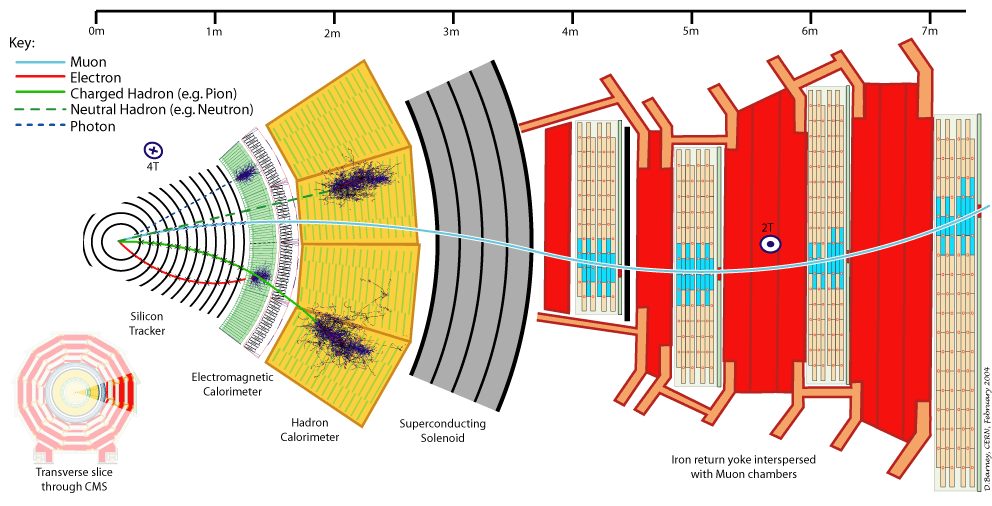
\includegraphics[width=0.9\textwidth]{./Figures/CMS_Slice.jpg}
  \caption{Cross Section of CMS showing the paths of various particle types through different segments of the detector \cite{cmsslice}}
  \label{CMS_SLICE}
\end{figure}

A cross section of CMS is shown in figure \ref{CMS_SLICE}. The coordinate system used by CMS takes the origin at the collision point. The z-axis points along the beam direction and defines the azimuthal angle, $\phi$. The psuedorapidity is defined by the polar angle, $\theta$, as $\eta=-ln(tan(\theta/2))$. The coverage of CMS is $|\eta|<5$. Transverse energies and momenta ($E_T $ and $p_T$)  are defined perpendicular to the beam \cite{cmsiop}. 

Charged particle trajectories are measured by the silicon pixel and strip tracker \cite{siliconTDR} in order to find their momentum. The CMS tracker achieves $15\mu m$ accuracy and a 1\% resolution for a particle with momentum up to $p_T < 40GeV$ with coverage for $|\eta|<2.5$. Muons are measured in the range $|\eta|<2.4$ and a $p_T$ resolution from $1-5\%$ can be achieved for $p_T < 1Tev$. The ECAL measures the energy of incident photons and electrons with aresolution better than $0.5\%$ for $E_T > 100 GeV$. The barrel provides coverage up to $|\eta| < 1.4$ and is extended to $|\eta|<3$ by the endcap. The HCAL has coverage of $|\eta|<3.0$ \cite{hcal} and a resolution for $E_T > 100GeV$ of 11\%. When combined with the ECAL jets can be measured to a resolution of $\Delta E/E \approx 100 \%/\sqrt{E[GeV]} \oplus 5\%$.
Potentially useful events are selected by the Level 1 (L1) hardware trigger which reduces the data rate from $\mathcal{0}40MHz$ to $100kHz$. These events are then processed in the HLT which utilises all detector information to further reduce the rate to $\mathcal{O}1kHz$.
